\graphicspath{{images_low_res/}}

\section{Background of Research}
\label{sec:background}

\subsection{A Comparison of Methods for Screening Strain Fitness }

QFA and SGA are methods for fitness screening using cultures grown on solid agar, both of
which can be performed using a high-throughput protocol (sga ref) \cite{Banks2012}. SGA
uses pinned cultures of higher initial cell density than the dilute liquid cultures used
in QFA. Although SGA allows for more repeats per plate (1536 cultures vs 384 cultures in
QFA), more of the growth curve can be captured with QFA so fits of growth models are more
accurate (see Figure~\ref{fig:qfa_and_sga_growth_curves}).
Comparison of QFA and SGA cultures in Figure~\ref{fig:qfa_and_sga_growth_curves}c shows
how QFA cultures are composed of many individual colonies which increase in thickness,
whereas SGA cultures are composed of a single uniform colony which grows outwards. The
number of individual colonies in a QFA culture is high enough that lag and other
stochastic effects should average out.

Colonyzer \citep{Lawless2010}, a tool for automatic capture of growth curves from images
of both QFA and SGA plates, uses integrated optical density (IOD) as a proxy for cell
density. Figure~\ref{fig:qfa_curves}, courtesy of \citet{Banks2012}, shows an example of
308 growth curves captured by Colonyzer from a QFA plate. In many SGA studies, culture
area, rather than IOD, is used as a proxy for culture density (example
ref). \cite{Lawless2010} found that direct area measurements are more noisy than IOD
measurements and provide a worse fit to the logistic model. To prevent bias in comparison
of data from QFA and SGA we will use Colonyzer to take the more accurate IOD measurements
for both data types.

\end{multicols}
\graphicspath{{images_low_res/}}
\begin{Figure}
  \centering
  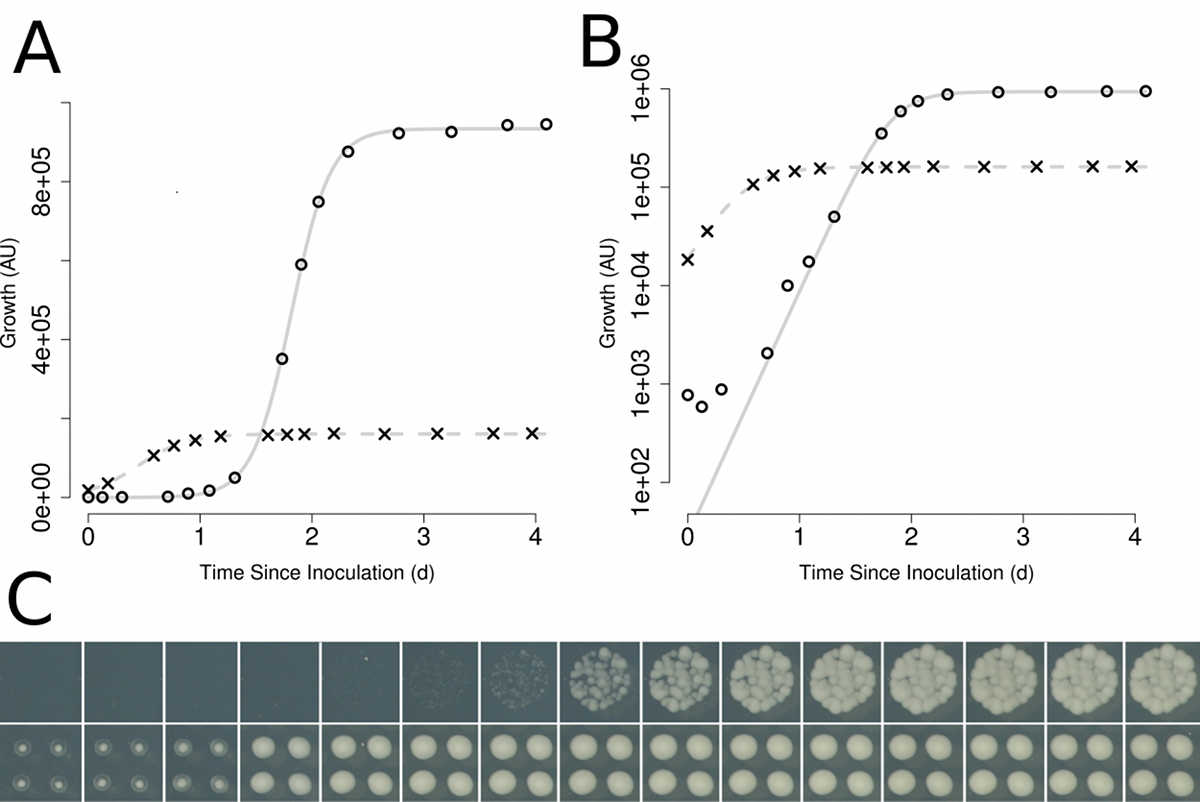
\includegraphics[width=\linewidth]{pin_v_spot_growth}
  \captionof{figure}{Fits of the logistic growth model, to cell
    density observations of yeast growing on solid agar, for spotted
    cultures (circles) and pinned cultures (crosses). In A) culture
    density is plotted on a linear scale. In B) culture density is
    plotted on a logarithmic scale. C) shows images of the spotted and
    pinned cultures corresponding to the data in A) \& B). Reproduced
    ??with permission?? from \citet{Lawless2010}.}
  \label{fig:qfa_and_sga_growth_curves}
\end{Figure}
\begin{multicols}{2}


\end{multicols}
\graphicspath{{images_low_res/}}
\begin{Figure}
  \centering
  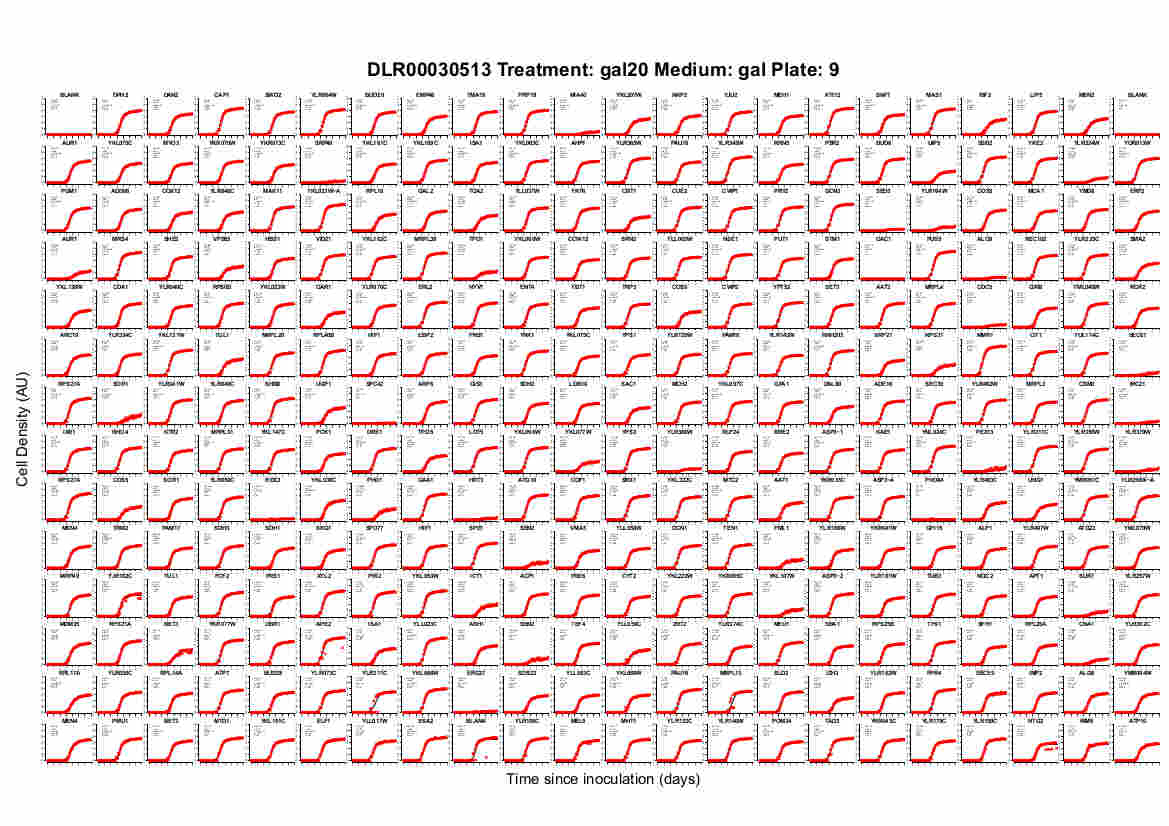
\includegraphics[width=\linewidth]{qfa_growth_array}
  \captionof{figure}{Growth curves, captured automatically by
    Colonyzer \citep{Lawless2010}, of 308 cultures in a QFA
    procedure. Reproduced ??with permission?? from \citet{Banks2012}.}
  \label{fig:qfa_curves}
\end{Figure}
\begin{multicols}{2}


\subsection{Competition and Signalling}

ethanol poisoning
quorum sensing

Fitness screening can also be performed using liquid cultures which are not susceptible to
competition or signalling effects. However, this approach has lower throughput (ref).

\begin{Figure}
  \centering
  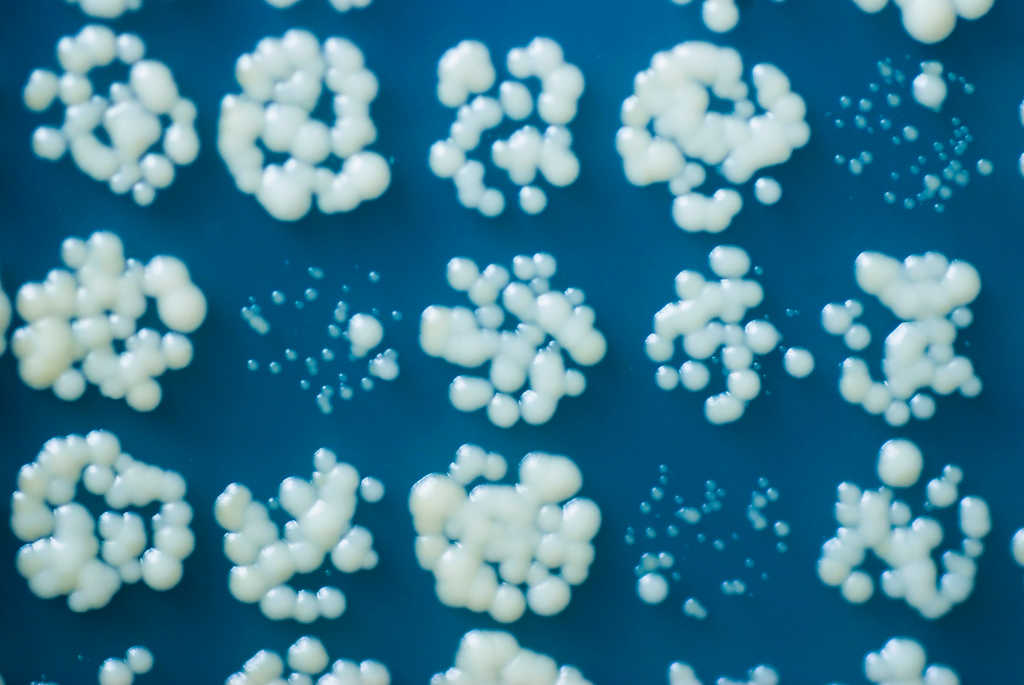
\includegraphics[width=\linewidth]{5658435523_c2e43729f1_b}
  \captionof{figure}{An image of 15 cultures on a section of solid agar
    from a QFA procedure. Image taken ??with permission?? from the Colonyzer GitHub repo
    https://github.com/CnrLwlss/Colonyzer \citep{Lawless2010}}
\end{Figure}

\subsection{Modelling Approaches}

\subsubsection{Mass Action Kinetics}
\subsubsection{The Logistic Growth Model}

The logistic growth model \cite{Verhulst1845} describes
\begin{equation}
  \label{eq:1}
  \dot{x} = rx\left(1 - \frac{x}{Z}\right)
\end{equation}
\subsubsection{Fishers multiplicative model of genetic interactions}
\subsubsection{Hierarchical models and Bayesian inference}

\subsection{Inference of Genetic Interactions / Telomere Cap Defects}
\label{sec:genetic-interaction}
(Move to background section.
Motivated by the link between telomere shortening, ageing, and cancer
(refs?), \citet{Addinall2011} study the genetic interactions of
\textit{cdc13} which functions in telomere capping in the model
organism \textit{Saccharomyces cerevisiae}. If the power to predict
genetic interactions is improved in the reanalysis of data from
\citet{Addinall2011}, this may highlight new genes involved in these
processes and will also be relevant for investigations of other types
of genetic interaction and investigations using other types of
microbial organism.)


%%% Local Variables:
%%% mode: latex
%%% TeX-master: "proposal"
%%% End:
